\documentclass{standalone}
\usepackage{tikz}
\usetikzlibrary{patterns, positioning}
\usepackage[sfdefault]{ClearSans} %% option 'sfdefault' activates Clear Sans as the default text font
\usepackage[T1]{fontenc}

\begin{document}
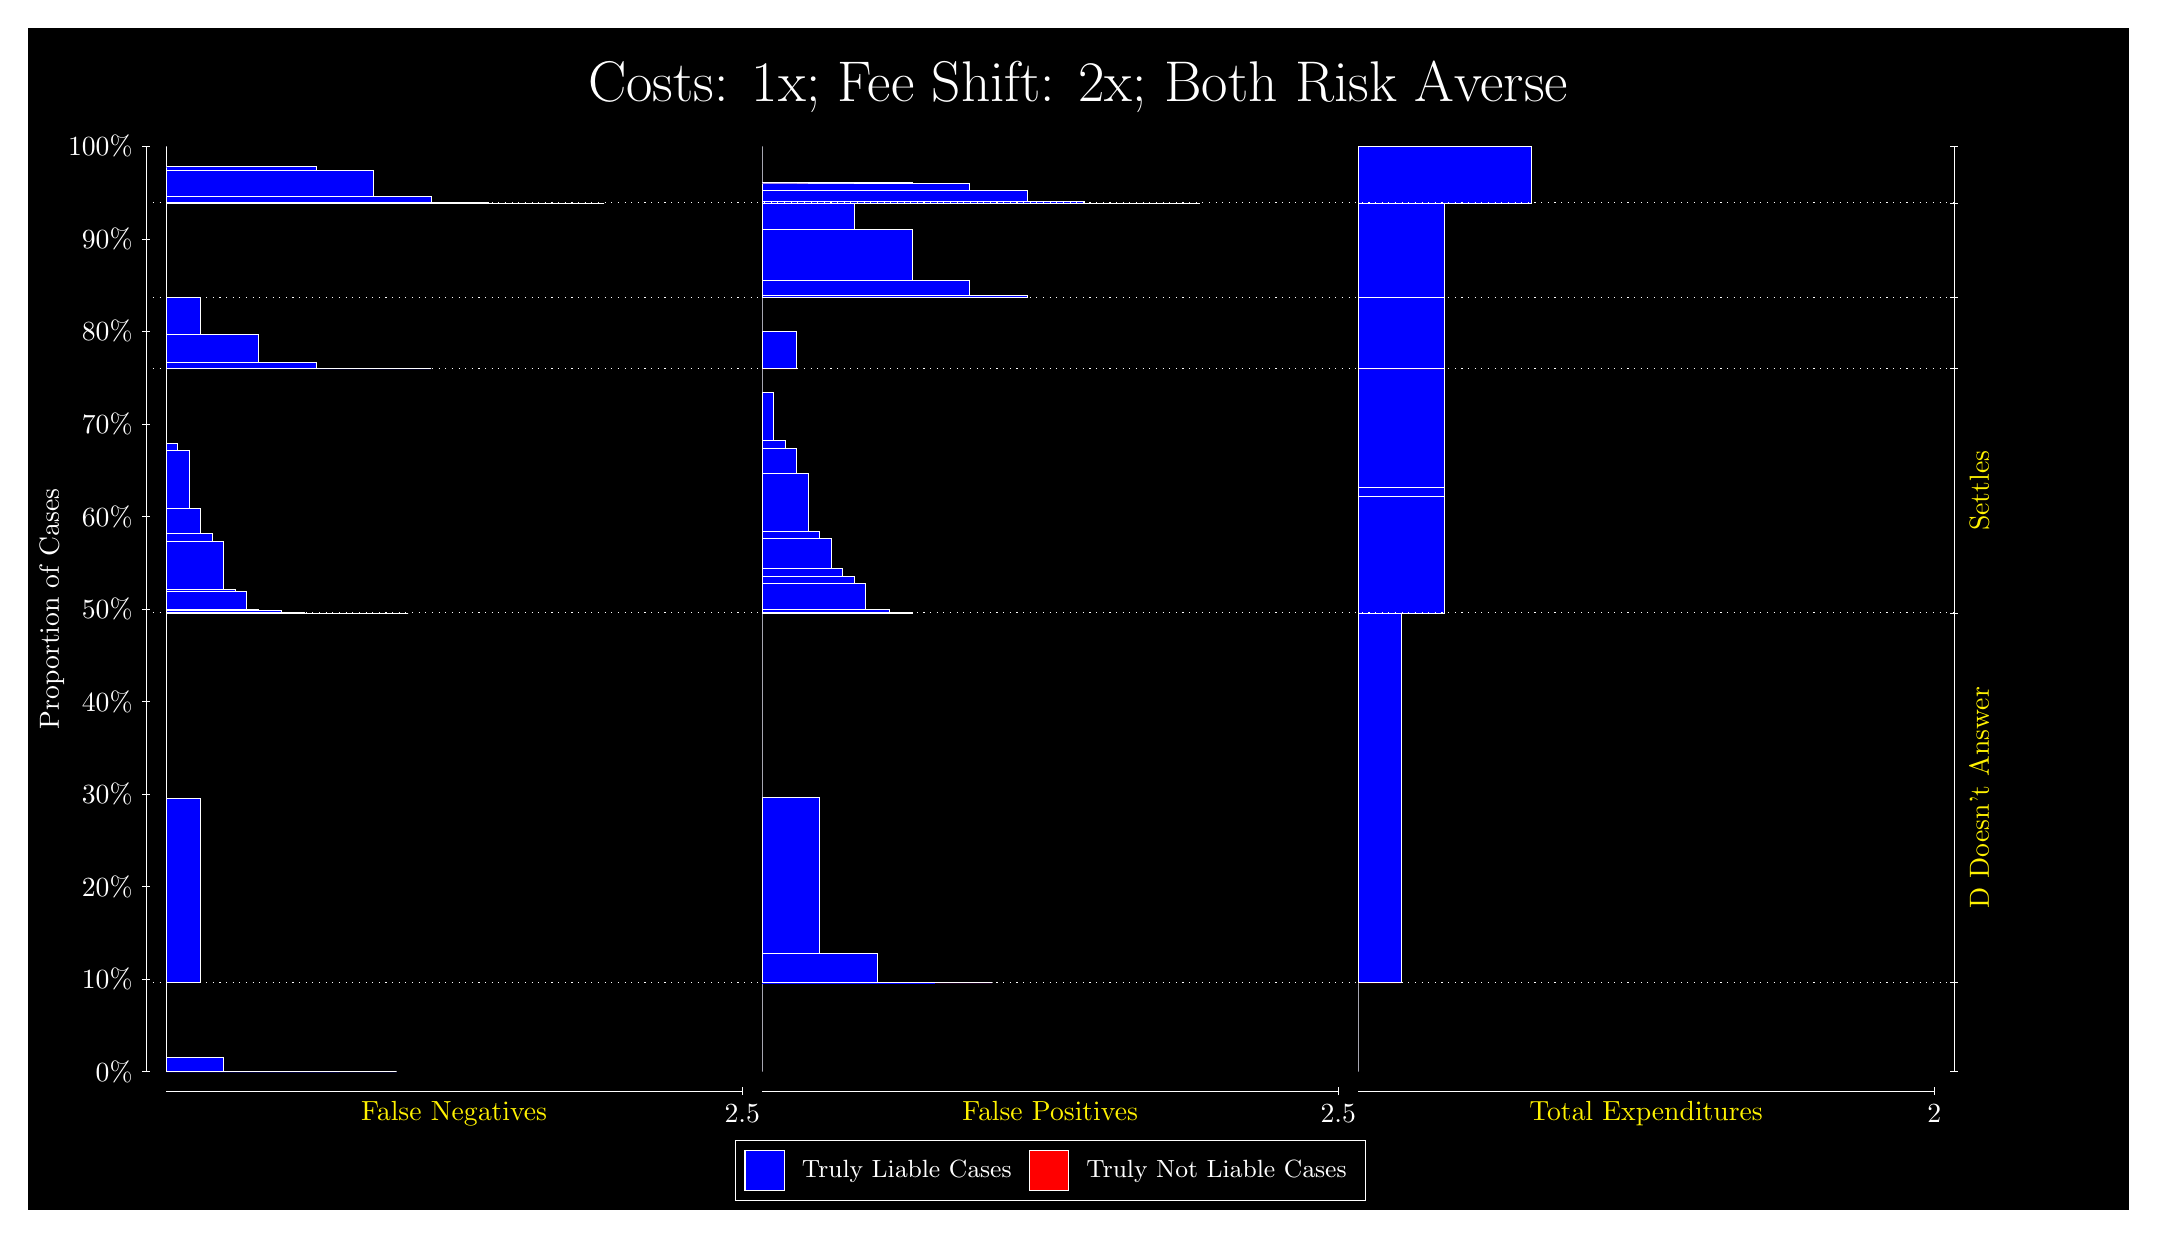
\begin{tikzpicture}
\draw[fill=black] (0,0) rectangle (26.667,15);
\draw[text=white] (0,13.5) rectangle (26.667,15) node[midway] {\huge Costs: 1x; Fee Shift: 2x; Both Risk Averse};
\draw[white, very thin] (1.5,1.75) -- (1.5,13.5);
\node[rotate=90, text=white, anchor=center] at (0.3, 7.625) {Proportion of Cases};
\draw[white, very thin] (1.45,1.75) -- (1.55,1.75);
\node[text=white, anchor=east] at (1.45, 1.75) {0\%};
\draw[white, very thin] (1.45,2.925) -- (1.55,2.925);
\node[text=white, anchor=east] at (1.45, 2.925) {10\%};
\draw[white, very thin] (1.45,4.1) -- (1.55,4.1);
\node[text=white, anchor=east] at (1.45, 4.1) {20\%};
\draw[white, very thin] (1.45,5.275) -- (1.55,5.275);
\node[text=white, anchor=east] at (1.45, 5.275) {30\%};
\draw[white, very thin] (1.45,6.45) -- (1.55,6.45);
\node[text=white, anchor=east] at (1.45, 6.45) {40\%};
\draw[white, very thin] (1.45,7.625) -- (1.55,7.625);
\node[text=white, anchor=east] at (1.45, 7.625) {50\%};
\draw[white, very thin] (1.45,8.8) -- (1.55,8.8);
\node[text=white, anchor=east] at (1.45, 8.8) {60\%};
\draw[white, very thin] (1.45,9.975) -- (1.55,9.975);
\node[text=white, anchor=east] at (1.45, 9.975) {70\%};
\draw[white, very thin] (1.45,11.15) -- (1.55,11.15);
\node[text=white, anchor=east] at (1.45, 11.15) {80\%};
\draw[white, very thin] (1.45,12.325) -- (1.55,12.325);
\node[text=white, anchor=east] at (1.45, 12.325) {90\%};
\draw[white, very thin] (1.45,13.5) -- (1.55,13.5);
\node[text=white, anchor=east] at (1.45, 13.5) {100\%};

\draw[white, very thin] (24.457,1.75) -- (24.457,13.5);
\draw[white, very thin] (24.407,1.75) -- (24.507,1.75);
\node[anchor=west] at (24.407, 1.75) {};
\draw[white, very thin] (24.407,2.8772) -- (24.507,2.8772);
\node[anchor=west] at (24.407, 2.8772) {};
\draw[white, very thin] (24.407,7.5756) -- (24.507,7.5756);
\node[anchor=west] at (24.407, 7.5756) {};
\draw[white, very thin] (24.407,10.677) -- (24.507,10.677);
\node[anchor=west] at (24.407, 10.677) {};
\draw[white, very thin] (24.407,11.582) -- (24.507,11.582);
\node[anchor=west] at (24.407, 11.582) {};
\draw[white, very thin] (24.407,12.782) -- (24.507,12.782);
\node[anchor=west] at (24.407, 12.782) {};
\draw[white, very thin] (24.407,13.5) -- (24.507,13.5);
\node[anchor=west] at (24.407, 13.5) {};

\draw[white, very thin, fill=blue] (1.75,1.75) rectangle (4.6775,1.75);
\draw[white, very thin, fill=blue] (1.75,1.75) rectangle (3.9457,1.75);
\draw[white, very thin, fill=blue] (1.75,1.75) rectangle (3.2138,1.7516);
\draw[white, very thin, fill=blue] (1.75,1.7516) rectangle (2.4819,1.9346);
\draw[white, very thin, fill=red] (1.75,1.9346) rectangle (1.75,1.9346);
\draw[white, very thin, fill=blue] (1.75,1.9346) rectangle (1.75,2.8772);
\draw[white, very thin, fill=blue] (1.75,2.8772) rectangle (2.1891,5.2234);
\draw[white, very thin, fill=red] (1.75,5.2234) rectangle (1.75,5.2234);
\draw[white, very thin, fill=blue] (1.75,5.2234) rectangle (1.75,7.5756);
\draw[white, very thin, fill=blue] (1.75,7.5756) rectangle (4.8239,7.5756);
\draw[white, very thin, fill=blue] (1.75,7.5756) rectangle (4.5312,7.5756);
\draw[white, very thin, fill=blue] (1.75,7.5756) rectangle (4.2384,7.5756);
\draw[white, very thin, fill=blue] (1.75,7.5756) rectangle (4.092,7.5756);
\draw[white, very thin, fill=blue] (1.75,7.5756) rectangle (3.9457,7.5756);
\draw[white, very thin, fill=blue] (1.75,7.5756) rectangle (3.7993,7.5756);
\draw[white, very thin, fill=blue] (1.75,7.5756) rectangle (3.6529,7.5756);
\draw[white, very thin, fill=blue] (1.75,7.5756) rectangle (3.5065,7.5798);
\draw[white, very thin, fill=blue] (1.75,7.5798) rectangle (3.3602,7.5802);
\draw[white, very thin, fill=blue] (1.75,7.5802) rectangle (3.2138,7.6038);
\draw[white, very thin, fill=blue] (1.75,7.6038) rectangle (3.0674,7.6116);
\draw[white, very thin, fill=blue] (1.75,7.6116) rectangle (2.921,7.6259);
\draw[white, very thin, fill=blue] (1.75,7.6259) rectangle (2.7746,7.8505);
\draw[white, very thin, fill=blue] (1.75,7.8505) rectangle (2.6283,7.8746);
\draw[white, very thin, fill=blue] (1.75,7.8746) rectangle (2.4819,8.4842);
\draw[white, very thin, fill=blue] (1.75,8.4842) rectangle (2.3355,8.5908);
\draw[white, very thin, fill=blue] (1.75,8.5908) rectangle (2.1891,8.8998);
\draw[white, very thin, fill=blue] (1.75,8.8998) rectangle (2.0428,9.6388);
\draw[white, very thin, fill=blue] (1.75,9.6388) rectangle (1.8964,9.7256);
\draw[white, very thin, fill=red] (1.75,9.7256) rectangle (1.75,9.7256);
\draw[white, very thin, fill=blue] (1.75,9.7256) rectangle (1.75,10.677);
\draw[white, very thin, fill=blue] (1.75,10.677) rectangle (5.1167,10.677);
\draw[white, very thin, fill=blue] (1.75,10.677) rectangle (4.3848,10.679);
\draw[white, very thin, fill=blue] (1.75,10.679) rectangle (3.6529,10.761);
\draw[white, very thin, fill=blue] (1.75,10.761) rectangle (2.921,11.109);
\draw[white, very thin, fill=blue] (1.75,11.109) rectangle (2.1891,11.582);
\draw[white, very thin, fill=red] (1.75,11.582) rectangle (1.75,11.582);
\draw[white, very thin, fill=blue] (1.75,11.582) rectangle (2.1891,11.586);
\draw[white, very thin, fill=red] (1.75,11.586) rectangle (1.75,11.586);
\draw[white, very thin, fill=blue] (1.75,11.586) rectangle (1.75,12.782);
\draw[white, very thin, fill=blue] (1.75,12.782) rectangle (7.3123,12.782);
\draw[white, very thin, fill=blue] (1.75,12.782) rectangle (6.5805,12.782);
\draw[white, very thin, fill=blue] (1.75,12.782) rectangle (5.8486,12.785);
\draw[white, very thin, fill=blue] (1.75,12.785) rectangle (5.1167,12.867);
\draw[white, very thin, fill=blue] (1.75,12.867) rectangle (4.3848,13.195);
\draw[white, very thin, fill=blue] (1.75,13.195) rectangle (3.6529,13.242);
\draw[white, very thin, fill=blue] (1.75,13.242) rectangle (3.0674,13.242);
\draw[white, very thin, fill=blue] (1.75,13.242) rectangle (2.921,13.242);
\draw[white, very thin, fill=blue] (1.75,13.242) rectangle (2.3355,13.242);
\draw[white, very thin, fill=red] (1.75,13.242) rectangle (1.75,13.242);
\draw[white, very thin, fill=blue] (1.75,13.242) rectangle (1.75,13.5);
\draw[white, very thin, fill=red] (9.3189,1.75) rectangle (9.3189,1.75);
\draw[white, very thin, fill=blue] (9.3189,1.75) rectangle (9.3189,2.8772);
\draw[white, very thin, fill=red] (9.3189,2.8772) rectangle (12.246,2.8772);
\draw[white, very thin, fill=blue] (9.3189,2.8772) rectangle (12.246,2.8772);
\draw[white, very thin, fill=blue] (9.3189,2.8772) rectangle (11.515,2.8802);
\draw[white, very thin, fill=blue] (9.3189,2.8802) rectangle (10.783,3.2528);
\draw[white, very thin, fill=blue] (9.3189,3.2528) rectangle (10.051,5.2294);
\draw[white, very thin, fill=blue] (9.3189,5.2294) rectangle (9.3189,7.5756);
\draw[white, very thin, fill=red] (9.3189,7.5756) rectangle (11.222,7.5756);
\draw[white, very thin, fill=blue] (9.3189,7.5756) rectangle (11.222,7.5852);
\draw[white, very thin, fill=red] (9.3189,7.5852) rectangle (10.929,7.5852);
\draw[white, very thin, fill=blue] (9.3189,7.5852) rectangle (10.929,7.6196);
\draw[white, very thin, fill=red] (9.3189,7.6196) rectangle (10.636,7.6196);
\draw[white, very thin, fill=blue] (9.3189,7.6196) rectangle (10.636,7.9526);
\draw[white, very thin, fill=blue] (9.3189,7.9526) rectangle (10.49,8.044);
\draw[white, very thin, fill=red] (9.3189,8.044) rectangle (10.344,8.044);
\draw[white, very thin, fill=blue] (9.3189,8.044) rectangle (10.344,8.1362);
\draw[white, very thin, fill=blue] (9.3189,8.1362) rectangle (10.197,8.5275);
\draw[white, very thin, fill=red] (9.3189,8.5275) rectangle (10.051,8.5275);
\draw[white, very thin, fill=blue] (9.3189,8.5275) rectangle (10.051,8.6143);
\draw[white, very thin, fill=blue] (9.3189,8.6143) rectangle (9.9044,9.3533);
\draw[white, very thin, fill=blue] (9.3189,9.3533) rectangle (9.758,9.6623);
\draw[white, very thin, fill=blue] (9.3189,9.6623) rectangle (9.6116,9.7688);
\draw[white, very thin, fill=blue] (9.3189,9.7688) rectangle (9.4652,10.378);
\draw[white, very thin, fill=blue] (9.3189,10.378) rectangle (9.3189,10.677);
\draw[white, very thin, fill=red] (9.3189,10.677) rectangle (9.758,10.677);
\draw[white, very thin, fill=blue] (9.3189,10.677) rectangle (9.758,11.151);
\draw[white, very thin, fill=blue] (9.3189,11.151) rectangle (9.3189,11.582);
\draw[white, very thin, fill=red] (9.3189,11.582) rectangle (12.686,11.582);
\draw[white, very thin, fill=blue] (9.3189,11.582) rectangle (12.686,11.609);
\draw[white, very thin, fill=blue] (9.3189,11.609) rectangle (11.954,11.801);
\draw[white, very thin, fill=blue] (9.3189,11.801) rectangle (11.222,12.45);
\draw[white, very thin, fill=blue] (9.3189,12.45) rectangle (10.49,12.779);
\draw[white, very thin, fill=blue] (9.3189,12.779) rectangle (9.758,12.782);
\draw[white, very thin, fill=red] (9.3189,12.782) rectangle (14.881,12.782);
\draw[white, very thin, fill=blue] (9.3189,12.782) rectangle (14.881,12.782);
\draw[white, very thin, fill=red] (9.3189,12.782) rectangle (14.149,12.782);
\draw[white, very thin, fill=blue] (9.3189,12.782) rectangle (14.149,12.783);
\draw[white, very thin, fill=red] (9.3189,12.783) rectangle (13.417,12.783);
\draw[white, very thin, fill=blue] (9.3189,12.783) rectangle (13.417,12.801);
\draw[white, very thin, fill=red] (9.3189,12.801) rectangle (12.686,12.801);
\draw[white, very thin, fill=blue] (9.3189,12.801) rectangle (12.686,12.947);
\draw[white, very thin, fill=blue] (9.3189,12.947) rectangle (11.954,13.036);
\draw[white, very thin, fill=blue] (9.3189,13.036) rectangle (11.222,13.04);
\draw[white, very thin, fill=blue] (9.3189,13.04) rectangle (10.49,13.04);
\draw[white, very thin, fill=red] (9.3189,13.04) rectangle (9.9044,13.04);
\draw[white, very thin, fill=blue] (9.3189,13.04) rectangle (9.9044,13.04);
\draw[white, very thin, fill=blue] (9.3189,13.04) rectangle (9.758,13.04);
\draw[white, very thin, fill=red] (9.3189,13.04) rectangle (9.3189,13.04);
\draw[white, very thin, fill=blue] (9.3189,13.04) rectangle (9.3189,13.5);
\draw[white, very thin, fill=red] (16.888,1.75) rectangle (16.888,1.75);
\draw[white, very thin, fill=blue] (16.888,1.75) rectangle (16.888,2.8772);
\draw[white, very thin, fill=red] (16.888,2.8772) rectangle (17.437,2.8772);
\draw[white, very thin, fill=blue] (16.888,2.8772) rectangle (17.437,7.5756);
\draw[white, very thin, fill=red] (16.888,7.5756) rectangle (17.986,7.5756);
\draw[white, very thin, fill=blue] (16.888,7.5756) rectangle (17.986,9.0588);
\draw[white, very thin, fill=red] (16.888,9.0588) rectangle (17.986,9.0588);
\draw[white, very thin, fill=blue] (16.888,9.0588) rectangle (17.986,9.1701);
\draw[white, very thin, fill=red] (16.888,9.1701) rectangle (17.986,9.1701);
\draw[white, very thin, fill=blue] (16.888,9.1701) rectangle (17.986,10.677);
\draw[white, very thin, fill=red] (16.888,10.677) rectangle (17.986,10.677);
\draw[white, very thin, fill=blue] (16.888,10.677) rectangle (17.986,11.582);
\draw[white, very thin, fill=red] (16.888,11.582) rectangle (17.986,11.582);
\draw[white, very thin, fill=blue] (16.888,11.582) rectangle (17.986,12.782);
\draw[white, very thin, fill=red] (16.888,12.782) rectangle (19.083,12.782);
\draw[white, very thin, fill=blue] (16.888,12.782) rectangle (19.083,13.5);
\draw[white, dotted] (1.5,2.8772) -- (24.457,2.8772);
\draw[white, dotted] (1.5,7.5756) -- (24.457,7.5756);
\draw[white, dotted] (1.5,10.677) -- (24.457,10.677);
\draw[white, dotted] (1.5,11.582) -- (24.457,11.582);
\draw[white, dotted] (1.5,12.782) -- (24.457,12.782);
\draw[white, very thin] (1.75,1.5) -- (9.0689,1.5);
\node[text=yellow, anchor=north] at (5.4094, 1.5) {False Negatives};
\draw[white, very thin] (9.0689,1.45) -- (9.0689,1.55);
\node[text=white, anchor=north] at (9.0689, 1.45) {2.5};

\draw[white, very thin] (9.3189,1.5) -- (16.638,1.5);
\node[text=yellow, anchor=north] at (12.978, 1.5) {False Positives};
\draw[white, very thin] (16.638,1.45) -- (16.638,1.55);
\node[text=white, anchor=north] at (16.638, 1.45) {2.5};

\draw[white, very thin] (16.888,1.5) -- (24.207,1.5);
\node[text=yellow, anchor=north] at (20.547, 1.5) {Total Expenditures};
\draw[white, very thin] (24.207,1.45) -- (24.207,1.55);
\node[text=white, anchor=north] at (24.207, 1.45) {2};


\node[text=yellow, centered, rotate=90] at (24.777, 5.2264) {D Doesn't Answer};
\node[text=yellow, centered, rotate=90] at (24.777, 9.1265) {Settles};




\draw (12.978300999999998,1.5) node[draw=none] (baseCoordinate) {};
\begin{scope}[align=center]
        \matrix[scale=0.5, draw=white, below=0.5cm of baseCoordinate, nodes={draw}, column sep=0.1cm]{
            \node[rectangle, draw, minimum width=0.5cm, minimum height=0.5cm, fill=blue] {}; &
            \node[draw=none, font=\small, text=white] (B) {Truly Liable Cases}; &
            \node[rectangle, draw, minimum width=0.5cm, minimum height=0.5cm, fill=red] {}; &
            \node[draw=none, font=\small, text=white] (B) {Truly Not Liable Cases}; \\
            };
\end{scope}

\end{tikzpicture}
\end{document}